\section{検証結果}
V字モデルに従って、実装部分に関するテストを行った。次に、それぞれに対してテストを行うことで、要件を満たしているかどうかを確認した。以下にそれぞれのテストの項目結果を表で示す。

\subsection{単体テスト}
V字モデルに従い,詳細設計を満たしているかどうかを確認する.まず,各種センサが要件を満たすかどうか検証した.次に,各種センサのテスト項目に従い,単体テストを行った.単体テストの第一段階として,確認内容の頭に*印のついていないテスト項目の機能テストを行った.*印のついているテスト項目については LED の点灯に関するものであり,追加を優先する機能ではないと判断し,第二段階のテストに含めた.

\subsection*{サーバ通信}
サーバ通信の検証で行った単体テストの項目を以下の表\ref{server_test_result}に示す。
\begin{table}[htbp]
\centering
\caption{サーバ通信単体テストの項目}
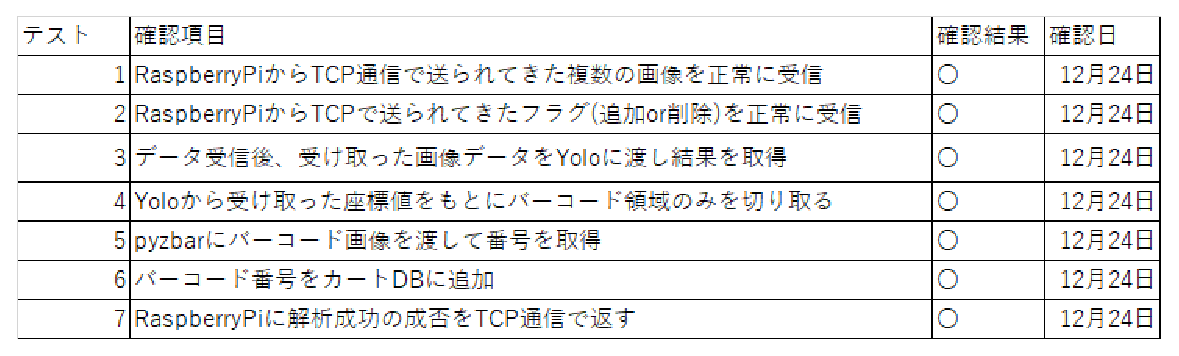
\includegraphics[width=14cm]{./pic/result/server_test_result.eps}
\label{server_test_result}
\end{table}

カゴクラスが解析に必要な、画像データとフラグ(追加・削除)を送信すると、解析システムがデータを受信して解析が始まる。画像データからバーコード番号の解析に成功すると、一緒に受信したフラグを使用して、カゴDBにバーコード番号を追加する。ただし、存在しない番号の追加を防ぐために、DBに追加する前に商品DBを参照し、該当するバーコード番号が存在する場合のみ追加を行う。また解析に成功した場合も、失敗した場合もカゴへ結果を送信する。

\subsection*{Yoloによるバーコード領域検知}
Yoloにおけるバーコード領域検知の検証で行った、単体テストの項目を以下の表\ref{yolo_test_result}に示す。

\begin{table}[htbp]
\centering
\caption{Yoloによるバーコード領域検知単体テストの項目}
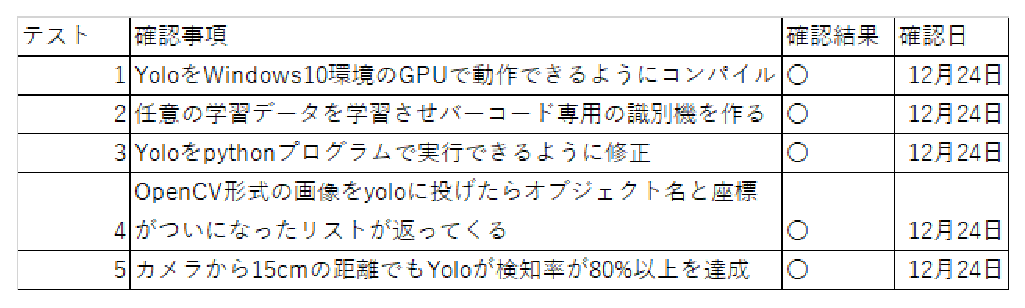
\includegraphics[width=14cm]{./pic/result/yolo_test_result.eps}
\label{yolo_test_result}
\end{table}

\newpage

\subsection*{DBを使用した商品情報の管理}
DBを使用した、商品情報の管理の単体テストの項目を以下の表\ref{table_test_result}に示す。

\begin{table}[htbp]
\centering
\caption{DBテーブル単体テストの項目}
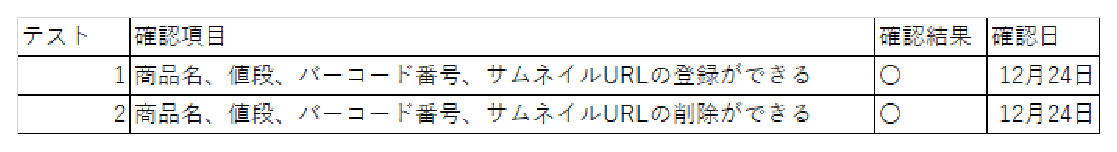
\includegraphics[width=15cm]{./pic/result/table_test_result.eps}
\label{table_test_result}
\end{table}

この商品DBは、店側が新商品の追加や、値段の更新を行いたい場合に操作される。

\subsection*{決済システム}
決済システムにおける単体テストの項目を、以下の表\ref{db_test_result}に示す。

\begin{table}[htbp]
\centering
\caption{決済システム単体テストの項目}
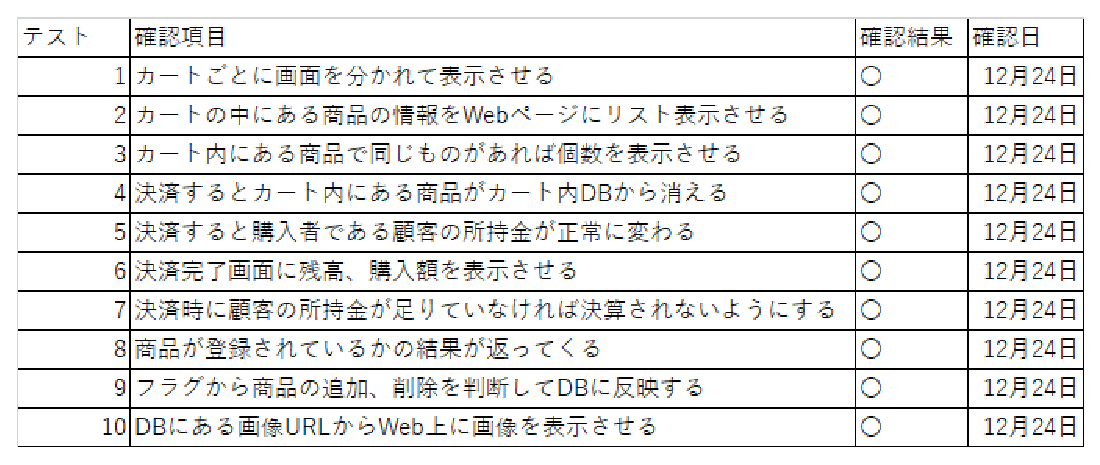
\includegraphics[width=15cm]{./pic/result/db_test_result.eps}
\label{db_test_result}
\end{table}

決済システムは、ユーザが決済を行うときに動作する。ユーザが商品を出し入れする時点で、購入予定商品の情報がカゴDBに格納されているため、決済時にカゴの中にある商品を1つずつスキャンする必要はない。

\newpage


\subsection{結合テスト}

これらの単体テストの項目を満たしていることを確認することで、商品識別システムが、表\ref{join_test_result}の結合テストの項目を満たしていることを確認する。結合テストでは、商品識別システムの中で筆者が実装を担当した、サーバ部分の項目が記されている。

\begin{table}[htbp]
\centering
\caption{結合テストの項目}
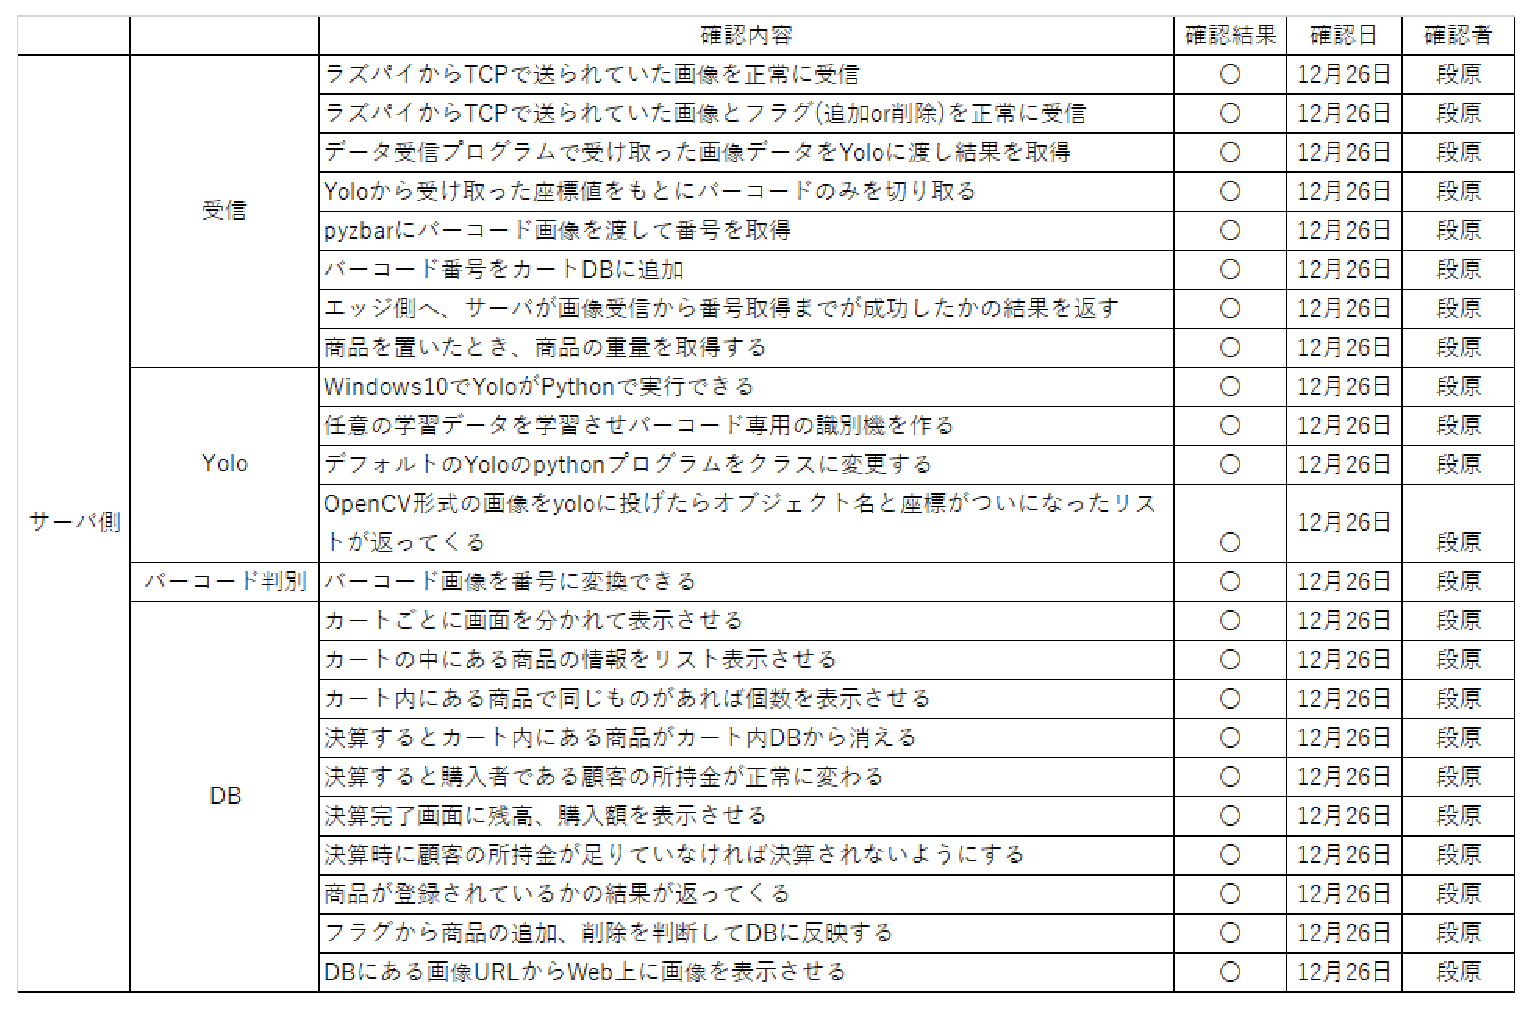
\includegraphics[height=15cm,width=15cm]{./pic/result/join_test_result.eps}
\label{join_test_result}
\end{table}

\newpage

\subsection{総合テスト}

結合テストの結果を確認し、各モジュール間でのデータの受け渡しが、正常に行われていることを確認した。最後に、表\ref{integrated_test_result}に総合テストの項目を示す。総合テストでは、ユーザが買い物を始めてから、決済するまでの流れをシナリオとしている。このシナリオでは、ユーザの残高は購入金額を下回らないと仮定する。また、決済前に買い物自体をキャンセルすることはないと仮定とした。

\begin{table}[htbp]
\centering
\caption{総合テストの項目}
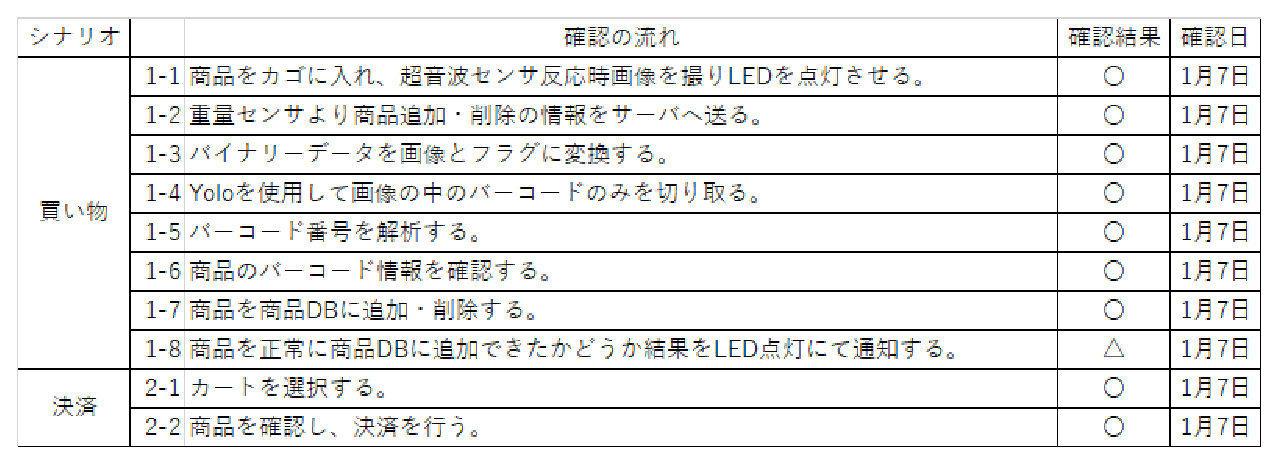
\includegraphics[width=15cm]{./pic/result/integrated_test_result.eps}
\label{integrated_test_result}
\end{table}